\chapter{Shrink}
\label{ch:shrinky}

Cílem této práce je analyzovat shrinky produktů, které byly zaznamenány v datech dané společnosti, a zjistit příčiny jejich vzniku. V následující části je vysvětlen pojem shrink a popsány kategorie, které vybraná společnost rozeznává ve svých datech.

\section{Definice}

Defince pojmu shrink v oblasti retailu není jednotná. Problematikou, jak přesně označit ztrátu produktů, se zabývá Beck ve svém článku \cite{bib:shrink2}. V této práci je slovem shrink označována ztráta zisku z neuskutečněného prodeje hotového produktu. Tento produkt je vyroben, či naskladněn, ale z nějakého důvodu nemohl být prodán zákazníkovi. Tímto důvodem může být například poničení produktu, jeho ztráta nebo prošlá doba spotřeby. Za shrink produktu lze označovat i stav, kdy cena produktu je neplánovaně snížena v důsledku zmíněných důvodů. Shrinkem je potom rozdíl plánované prodejní ceny a ceny, za kterou byl produkt skutečně prodán \cite{bib:DefShrink}. Tuto definici jsem zvolila vzhledem k povaze dat anlyzované společnosti.

Často se v literatuře lze setkat s pojmem shrink, resp. anglickým \emph{shrinkage} v retailových společnostech především v souvislosti se ztrátou zboží z~důvodu krádeže -- interní neboli zaměstnanecká, externí neboli zákaznická, dále z~důvodu administrativního pochybení, nebo podovodem na straně dodavatele. Vzhledem k~této časté definici shrinku se řada prací o shrincích věnuje možnostem zpřísnění bezpečnosti prodejen nebo lepšímu zabezpečení často kradeného zboží, aby bylo omezeno množství krádeží.\cite{bib:shrink1,bib:shrink2}


% Cílem každé společnosti by mělo být tyto shrinky minimalizovat, protože kvůli shrinkům firma přichází o zisk. 

\section{Typy shrinků}
\label{sec:shrinkyTypy}

Shrinky je možné kategorizovat podle Becka do čtyř kategorií podle čtyř oblasti, kde se shrink odehrává. Kategorie se dále dělí na ztráty, které jsou známé a neznámé. Neznámé ztráty z povahy věci nejde evidovat, takže se dále již nedělí. Známou ztrátu lze dále rozdělit na úmyslně a neumýslně zaviněnou. Rozdělení je podrobně znázorněno na obrázku \ref{obr:shrinkytypyBeck}.

\begin{figure}[hbtp!]
    \centering
    \captionsetup{justification=centering}
    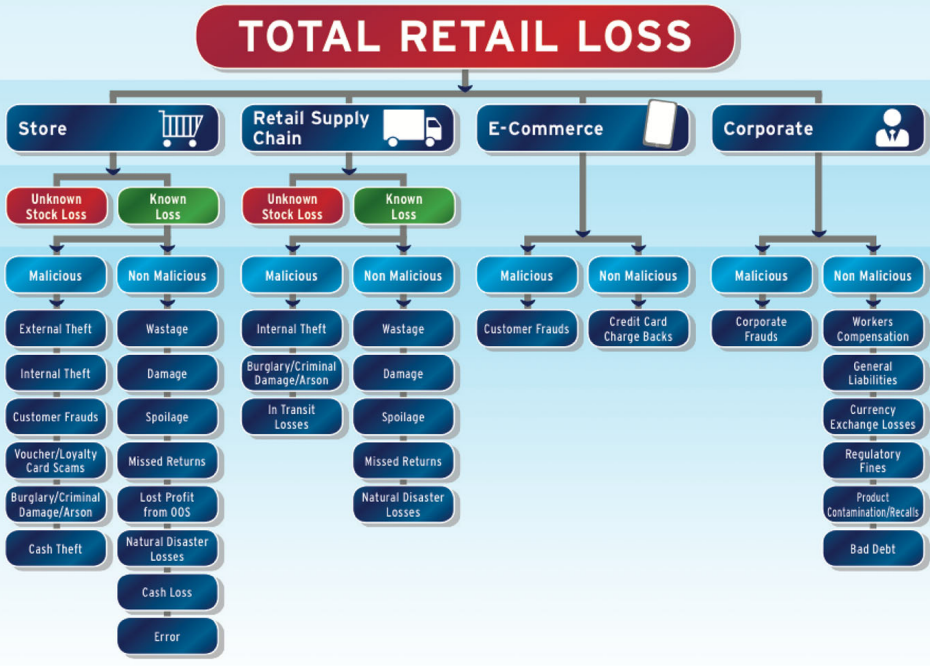
\includegraphics[width=\textwidth]{obrazky/typyshirnku.png}
    \caption{Topologie shrinků. Zdroj: \cite{bib:shrink2}}
    \label{obr:shrinkytypyBeck}
\end{figure}

Vybraná společnost rozlišuje ve svých datech tři kategorie shrinku -- shrinky způsobené inventurou, škodami a cenové snížení. Dále se text věnuje popisu jednotlivých typů v rámci těchto kategorií v analyzované společnosti. Každý typ má přiřazeno jednoznačné identifikační číslo, podle kterého je zaznamenáván v databázi. Z důvodů anonymizace dat v práci nejsou uvedené přesné hodnoty těchto ID, namísto toho jsou uvedeny pouze názvy, které definují shrinky.

\vspace*{1em}

\textbf{Shrinky způsobené inventurou}
Tato kategorie sdružuje všechny shrinky týkající se změn ve stavech zásob. Tyto změny se projeví při inventuře. V tabulce \ref*{tab:sh:inv} se nachází přehled všech evidovaných typů. Některé typy mají obdobný význam a jsou duplicitní. K tomu mohlo dajít patrnš tím, že některé subjekty používají dřívější značení pro inventuru, než jiné subjekty, které mohli přejít na nový, podorbnější způsob záznamu. 

\vspace*{1em}

\textbf{Shrinky způsobené škodami}

Do kategorie shrinků způsobených škodami jsou řazeny zbylé důvody k odstranění produktu z prodeje z důvodu degradace produktu. V následující tabulce \ref{tab:sh:dam} jsou vypsané všechny typy, které moho být evidovány.

\textbf{Snížení ceny}
 
Tento typ shrinku vzniká v důsledku snížení ceny na prodejně. Tento shrink není přímo evidovaný v datech, ale lze jej vypočítat ze záznamů prodejů. Jedná se o situaci, kdy přímo na prodejně je nějaký produkt zlevněný v důsledku blížící se expirace nebo z důvodu poničení obalu. Nejedná se tak o klasickou promoakci, ale o zlevnění, které není evidováno systémem, protože se netýká všech produktů daného typu, ale pouze jednoho či několika konkrétních produktů na vybrané prodejně.

Postup pro zjištění velikosti shrinku pro jeden konkrétní produkt je následovný. Pro každou účtenku je třeba porovnat cenu každého prodaného produktu s ceníkovou cenou, případně promoční slevou. Pokud si tyto ceny nejsou rovné, pak rozdíl těchto cen je shrink daného produktu.

Vzhledem k tomu, že denně se na každé prodejně zaevidují stovky účtenek, bylo by toto postupné procházení velmi časově náročné. Zároveň tento shrink postihuje jen velmi malou část celkového prodaného objemu. Tento shrink jsem ve svých analýzách již dále nezkoumala, protože nebyl shledán prioritním. Určení příčin vzniku takového shrinku se může lišit v závislosti na konkrétních prodejnách, a to jak na zaměstnaních, které vytváří snížení cen, tak na spotřebitelích, kteří na konkrétních prodejnách nakupují.

\begin{table}[hbtp!]
    \caption{Přehled jednotlivých typů shrinků  způsobených inventurou.}
    \label{tab:sh:inv}
    \begin{tabular}{ p{4cm} p{10.5cm}}
     Název             & Popis \\
    \hline
              Inventura - příjem           & Kladné připsání zboží během inventury.      \\
              Inventura - odpis           & Záporné odepsání zboží během inventury.      \\
              Inventura - velká             & Velká inventura skladu.     \\
              Inventury - oprava       & Dodatečné opravy, které bylo třeba provést po dokončení velké inventury.      \\
              Inventura - částečná    & Odpis, nebo naskladnění zboží při inventuře položek.      \\
              Neuznané reklamace \par centrálním skladem  \strut &  Odpis zboží, které bylo fyzicky dodané z centrálního skladu na prodejnu, ale prodejna jej vrátila, ale vratka nebyla uznána.     \\
              Inventura              & Starší verze ID používaného pro inventuru.\\
              Neexistující zboží     & Odpis prokazatelně ukradeného zboží nebo i ztraceného zboží.      \\
    \end{tabular}
\end{table}

\begin{table}[hbtp!]
    \caption{Přehled jednotlivých typů shrinků způsobených škodami.}
    \label{tab:sh:dam}
    \begin{tabular}{ p{4cm} p{10.5cm}}
         Název             & Popis \\
    \hline
                Poškození               & Odpis zboží, které bylo poškozené. Např. nedopečené, spálené, špatně vyrobené nebo poškozené zaměstnancem nebo zákazníkem (kdy nelze uplatnit reklamaci na zákazníka.)       \\
                Prošlé a zkažené zboží  & Odpis zboží, kterému prošla doba spotřeby (v případě výrobků, kde je datum uvedené), zkažené či shnilé zboží (ovoce, zelenina) nebo ztvrdlé pečivo.       \\
                Zákaznické \par reklamace \strut  & Odpis zboží, které zákazník reklamoval a reklamace byla uznána, ale zároveň nelze toto zboží reklamovat u dodavatele.      \\
                Reklamace \par centrálního skladu \strut   &  Odpis zboží, které fyzicky nedorazilo z distribučního centra a nebylo možné ho reklamovat z důvodu nesplnění limitu pro vytvoření reklamace na distribučním centru. Také obsahuje odpisy neprodaných položek po ukončení výprodeje.     \\
                Kompostéry              & Odpis zboží, které je prošlé nebo poškozené a které prodejna zlikviduje v kompostéru.       \\
                Potravinová banka       & Odpis potravinářského zboží, které bylo darováno potravinovým bankám. Jedná se o produkty, které nebylo možné zařadit znovu do oběhu.    \\
                Zvířecí útulky          & Odpis potravinářského zboží, které bylo darováno do útulků zvířat. Jedná se o produkty, které nebylo možné zařadit znovu do oběhu.          \\
                Poškození vnějšími \par vlivy \strut %(internal use (err)) 
                                        & Odpis zboží, které bylo poškozeno nebo zničeno vlivem třetí strany (výbuch, vytopení, poškození majetku) nebo přírodními živly. Zboží se tedy na prodejně nenachází a nemůže proto být zlikvidováno.      \\
                Zničení & Jinak zničené zboží \\
    \end{tabular}
\end{table}



\vspace*{1em}